\documentclass[10pt,a4paper]{article}

\usepackage[a4paper,top=0.85cm,bottom=0.85cm,left=1.05cm,right=1.05cm]{geometry}
\usepackage{fontspec}
\usepackage[french]{babel}
\usepackage[hidelinks]{hyperref}
\usepackage{xcolor}
\usepackage{graphicx}
\usepackage{titlesec}
\usepackage{enumitem}

\setmainfont{Arial}
\pagestyle{empty}
\setlength{\parindent}{0pt}
\setlength{\parskip}{0pt}
\linespread{0.96}
\hyphenpenalty=10000
\exhyphenpenalty=10000
\sloppy
\setlist[itemize]{leftmargin=1.05em,itemsep=0pt,topsep=1pt,parsep=0pt,label=-}
\urlstyle{same}

\definecolor{heading}{HTML}{123867}
\titleformat{\section}{\large\bfseries\color{heading}}{}{0pt}{}[\vspace{-5pt}\rule{\linewidth}{0.5pt}]
\titlespacing{\section}{0pt}{5pt}{3pt}

\newif\ifwithphoto
\withphotofalse
\IfFileExists{with_photo.flag}{\withphototrue}{}

\newcommand{\role}[3]{%
  \textbf{#1} \hfill #3\\
  \textit{#2}\vspace{1pt}
}

\newcommand{\edu}[4]{%
  \textbf{#1} -- #2 \hfill #3 #4\\[-1pt]
}

\begin{document}

\ifwithphoto
\begin{minipage}[c]{0.76\linewidth}
{\LARGE \textbf{Kossi Richard Allado}}\\
\textbf{Étudiant ingénieur en cybersécurité et IA | SOC, DFIR, pentest junior, IAM}\\
Beni Mellal, Maroc | +212 621 074 305 | \href{mailto:alladokossirichard2025@gmail.com}{alladokossirichard2025@gmail.com}\\
\href{https://allakori.github.io/}{https://allakori.github.io/}\\
\href{https://github.com/ALLAKORI}{https://github.com/ALLAKORI}\\
\href{https://www.linkedin.com/in/kossi-richard-allado-50177b2a5}{https://www.linkedin.com/in/kossi-richard-allado}\\
\href{https://tryhackme.com/p/RIDOKY}{https://tryhackme.com/p/RIDOKY}
\end{minipage}
\hfill
\begin{minipage}[c]{0.18\linewidth}
\raggedleft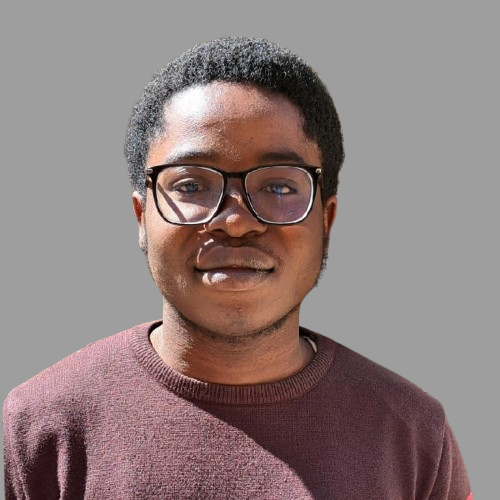
\includegraphics[width=2.35cm]{photo_richard.png}
\end{minipage}
\else
{\LARGE \textbf{Kossi Richard Allado}}\\
\textbf{Étudiant ingénieur en cybersécurité et IA | SOC, DFIR, pentest junior, IAM}\\
Beni Mellal, Maroc | +212 621 074 305 | \href{mailto:alladokossirichard2025@gmail.com}{alladokossirichard2025@gmail.com}\\
\href{https://allakori.github.io/}{https://allakori.github.io/}\\
\href{https://github.com/ALLAKORI}{https://github.com/ALLAKORI}\\
\href{https://www.linkedin.com/in/kossi-richard-allado-50177b2a5}{https://www.linkedin.com/in/kossi-richard-allado}\\
\href{https://tryhackme.com/p/RIDOKY}{https://tryhackme.com/p/RIDOKY}
\fi

\section{Profil}
Étudiant ingénieur en cybersécurité et IA à l'ENSA Beni Mellal, avec une pratique régulière de l'analyse de journaux, du durcissement Linux, de l'investigation d'incidents et des tests de sécurité applicative. Je construis des preuves techniques à travers des labs documentés, des write-ups CTF et des projets orientés remédiation, avec une approche rigoureuse de la collecte de traces et de la reproductibilité.

Je recherche un stage PFA en cybersécurité, SOC, DFIR, pentest junior, IAM ou sécurité systèmes/réseaux. Mon profil combine une base solide en Python et Linux, une aisance avec les outils d'analyse et une capacité à transformer des observations techniques en constats exploitables pour une équipe sécurité.

\section{Compétences techniques}
\textbf{SOC / DFIR :} corrélation de logs Linux et Windows, IOC, chronologie d'incident, analyse d'artefacts, journalisation, remédiation --- Splunk, auditd, Sysmon, Volatility, WinPMEM, Autopsy, FTK Imager.\\
\textbf{Sécurité offensive / web :} reconnaissance, énumération, exploitation contrôlée, preuve de concept, rédaction de write-ups --- Kali Linux, Nmap, Wireshark, Burp Suite, Hydra, SQL injection, XSS, DVWA.\\
\textbf{Systèmes / IAM :} durcissement Linux, gestion des accès, contrôle des privilèges, MFA et PKI --- SSH, UFW, Fail2ban, SELinux, AppArmor, Lynis, Keycloak, OpenSSL, RBAC.\\
\textbf{Programmation / données :} Python, Bash, C, SQL, Pandas, Scikit-learn, Tkinter, Jupyter, Git/GitHub.

\section{Projets techniques}
\textbf{Linux Server Compromise \& Forensic Investigation Lab} \hfill 2026\\
\href{https://github.com/ALLAKORI/Linux-Server-Compromise-Forensic-Investigation-Lab}{https://github.com/ALLAKORI/Linux-Server-Compromise-Forensic-Investigation-Lab}
\begin{itemize}
  \item Environnement multi-VM avec Kali Linux comme machine d'attaque et Ubuntu Server comme cible, en s'appuyant sur SSH, UFW, auditd et Fail2ban.
  \item Simulation contrôlée d'une compromission, puis analyse des connexions SSH, commandes, comptes créés, activités sudo et traces auditd.
  \item Remédiation documentée : blocage UFW, suppression du compte malveillant, réinitialisation des accès et durcissement des services exposés.
\end{itemize}

\textbf{Volt Typhoon Intrusion Investigation} \hfill 2026\\
\href{https://allakori.github.io/writeups/tryhackme/volt-typhoon/}{https://allakori.github.io/writeups/tryhackme/volt-typhoon/}
\begin{itemize}
  \item Analyse d'un scénario de type APT avec des journaux Windows et des phases MITRE ATT\&CK simulées dans un environnement TryHackMe.
  \item Mise en évidence d'abus de PowerShell, WMIC, certutil, netsh, web shell, Mimikatz et effacement de journaux.
  \item Production d'une chronologie, d'IOC et de requêtes d'investigation orientées détection et confinement.
\end{itemize}

\textbf{Identity, Access \& Application Security Labs} \hfill 2025\\
\href{https://github.com/ALLAKORI/cybersecurity-iam-labs}{https://github.com/ALLAKORI/cybersecurity-iam-labs}
\begin{itemize}
  \item Déploiement d'un laboratoire Linux/Keycloak pour gérer utilisateurs, rôles, RBAC et MFA/TOTP sur des scénarios d'accès.
  \item Exercices OpenSSL/PKI et DVWA pour analyser SQL injection et XSS, puis documenter les contre-mesures.
  \item Mise en pratique d'un raisonnement sécurité applicative avec preuves, risques et correctifs.
\end{itemize}

\textbf{CSIA CTF 2026 - 1ère place avec Team GHOSTSHELL} \hfill 2026\\
\href{https://github.com/ALLAKORI/csia-ctf-2026-writeups}{https://github.com/ALLAKORI/csia-ctf-2026-writeups}
\begin{itemize}
  \item Résolution en équipe de challenges web, OSINT, forensic et stéganographie avec rédaction de write-ups reproductibles.
\end{itemize}

\section{Expérience}
\role{Stagiaire IA / Maintenance prédictive}{ONEE - Branche Eau, Kasba Tadla}{Août 2025}
\begin{itemize}
  \item Préparation de données capteurs de pompe haute pression pour détecter des signaux de défaillance.
  \item Entraînement d'un modèle Random Forest avec Python, Pandas et Scikit-learn pour classifier un niveau de risque.
  \item Développement d'un prototype Tkinter pour tester les prédictions et exposer les résultats de manière exploitable.
\end{itemize}

\section{Formation}
\edu{Cycle ingénieur}{Cybersécurité et Intelligence Artificielle, ENSA Beni Mellal}{2024 -- Présent}{}
\edu{DEUST}{Mathématiques, Informatique, Physique, FST Fès}{2022 - 2024}{-- Mention Bien}
\edu{Baccalauréat scientifique}{Série D, Lycée de Djagblé, Togo}{2022}{-- Mention Très Bien}

\section{Certifications et réalisations}
Cisco Ethical Hacker | Google Cybersecurity : Foundations et Play It Safe | TryHackMe Junior Penetration Tester Learning Path | TryHackMe Advent of Cyber 2025 | Udemy Cryptography and Hashing | CSIA CTF 2026 : 1ère place

\section{Langues}
Français : courant | Anglais : professionnel technique | Éwé : langue maternelle

\end{document}
